\documentclass[a4paper, 11pt, twocolumn]{article}
\usepackage{caption}
\usepackage{graphicx}
\usepackage{color} %colors in text
\usepackage{textcomp} % 
\usepackage[T1]{pbsi} %hand writting nice 
\usepackage[T1]{fontenc} %more fonts
\usepackage{mathrsfs} % letters for math
\usepackage{fullpage} % no margins
\usepackage{amsmath} % math formulas
\usepackage[all]{xy} % for drawing
\usepackage{listings}
\usepackage{algorithmic}
\usepackage{algorithm}
\usepackage{amssymb}
\usepackage[parfill]{parskip}
%\usepackage{palatino, url, multicol} %multicolumns
\definecolor{gray}{rgb}{0.7,0.7,0.7} 
\usepackage{enumerate} %for enumerate
\fontfamily{cmbr}\selectfont\normalsize
\newcommand{\ds}{\displaystyle}
\newcommand{\todo}[1]{\textcolor{red}{\textbf{#1}}}
\newcommand{\fade}[1]{\textcolor{gray}{\textbf{#1}}}
%\hyphenpenalty=100000
\date{} % fara data
\author{\fade{Nimrod Raiman [0336696]}\\\fade{Silvia L. Pintea [6109960]}}
\title{Rock, Paper \& Scissors with Nao}
\begin{document}
    \maketitle
	%ABSTRACT SECTION__________________________________________
    \abstract{Throughout this paper we are going to explain our work on teaching a humanoid robot (\emph{Nao}) to play \emph{"Rock, paper \& scissors"}. In order to accomplish this task we have used different theoretical methods which are described in the section~\ref{sec:methods}. The next section presents our experimental results. Finally we give an overall view of this paper and indicate the possible future work that could be done on this subject.}  
	%SECTION SECTION_________________________________________
    \section{Introduction}
	\label{sec:intro}
        \emph{"Rock, Paper \& Scissors"} is an easy and well known game. This is the reason for which it is interesting to learn a robot how to play it against human players. In order to do that the robot needs to be able to recognize the hands of its opponent and classify the gesture as: \emph{"rock"}, \emph{"paper"} or \emph{"scissors"}.\\	
		\hspace*{10px}In this paper we describe our approach to accomplish this in real time. Our solution is fairly robust to lightning condition and also the gestures of the player need not be restricted to certain angles or positions in the frame.\\ 
        \hspace*{10px}Our problem has been split into three main tasks: extracting the hands from the webcam stream, recognizing the gesture of the extracted hand and implementing motion and speech on \emph{Nao}. Throughout our project we have tried different approaches in order to find the best method to solve the problem.\\
		 \hspace*{10px}We have experimented with methods such as: \emph{backprojection} of pixel values for hand detection, \emph{Gabor filters} and \emph{PCA} for classifying signs. We will start by describing the methods that we have tried and then continue by giving an overview of the results and the conclusions.   
	%METHODS SECTION__________________________________ 
    \section{Methods}
	\label{sec:methods}
		For hand detection and recognition we have employed two different techniques: a naive approach and the backproject of the pixels corresponding to skin.\\
		\hspace*{10px}For the gesture recognition we have experimented with different sets of data and we have extracted different features using methods such as: \emph{PCA} and \emph{Gabor filters}. We have also tried using two different types of classifiers: \emph{SVM} (support vector machine) and \emph{Knn} (K nearest neighbors).\\
		\hspace*{10px}We will continue by giving a more detailed description of the methods employed. 
        \subsection{Hands extraction}
		\label{sec:Meth_exrctHands}
        \subsubsection{Naive approach}
		\todo{Nimrod .....}\\

        \subsubsection{Backprojection of skin pixels}
        \todo{Nimrod .....}\\
        Determine hue and saturation values for skin color\\
        Threshold the image with hue and saturation values\\
        Use erosion \& dilation\\
        Find ares corresponding to hands\\
        vspace*{10px}
        Robust/sophisticated approach\\
        Determine skin color histogram\\
        - Detect face\\
        - Build histogram of pixels corresponding to the face\\
        Backproject skin color histogram on whole frame\\
        Use erosion \& dilation to reduce the noise and fill up gaps\\
        Extract area of corresponding to the hand\\
        Use more sophisticated erosion \& dilation on hand area\\
        - Retain the hand and remove the background\\
        - Resize the area of interest to 70x70

        \subsection{Gesture recognition}
		For the gesture recognition task we have started by using a training set containing images of hands of \emph{70$\times$70}px with different backgrounds. The problem proved to be too complex for our classifiers so we have decided to switch to a simpler one which would contain only centered hands and a black background.\\ 
		\hspace*{10px}Out of this dataset we have extracted the features to be used during the classification.
		\label{sec:Meth_clssifyHands}
		\subsubsection{PCA}
		The first technique we have tried was \emph{PCA}. We have computed the \emph{eigen-hands} of our data and then we have projected each set, separately, on this space.\\
		\hspace*{10px}There are three steps for generating the \emph{eigen-hands}:
		\begin{itemize}
		\item Subtracting the mean of the data
		\item Computing the covariance of the data and the eigenvectors of the covariance matrix
		\item Projecting each training set (corresponding to each sign: \emph{"rock"}, \emph{"paper"} or \emph{"scissors"}) on the space defined by the eigenvectors
		\end{itemize}
		\hspace*{10px}For high-dimensional data a better approach than computing the eigenvectors of the matrix: \emph{$Data^T \times Data$} (which for a dataset of \emph{[N,D]} with \emph{$D\gg N$} has the dimension \emph{[D,D]}) would be to use an intermediate step and compute the eigenvectors \emph{$V \rightarrow eigh(Data\times Data^T)$} and then determine the final \emph{eigen-space}: \emph{$U \rightarrow \frac{Data^T\times V}{norm(Data^T\times V)}$}.\\
		\hspace*{10px}Unfortunately, given the fact that \emph{PCA} is not background invariant, translation invariant or rotation invariant the results were not as good as we were expecting.	
		\subsubsection{Gabor filters}
		A \emph{Gabor wavelet} is created by defining the size of the wavelet to be generated and then by looping over the coordinates of each pixel (\emph{x} and \emph{y}) and applying the following formula:\\
		\begin{table}[!htbp]
		\begin{tabular}{| c |}
			\hline\\
	 		\emph{$ g(x,y,\lambda,\theta,\psi,\sigma,\gamma) = exp(-\frac{x\prime^2+\gamma^2y\prime^2}{2\sigma^2})cos(2\Pi\frac{x\prime}{\lambda}+\psi)$}\\[10px]
			where $x\prime$ = x cos$\theta$+y sin$\theta$\\
			and $y\prime$ = -x sin$\theta$+y cos$\theta$\\[2px]
			\hline
		\end{tabular}
		\end{table}

		The parameter $\lambda$ represents the frequency of the stripes in the wavelet, $\theta$ gives the angle of the stripes, $\psi$ is a translation parameter, $\sigma$ gives the size of the stripes while $\gamma$ indicates how elliptical they are.\\  
		\begin{figure}[!hbtp]
		   \centering
		   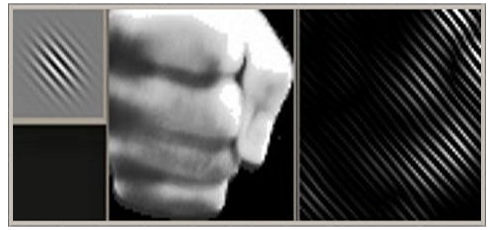
\includegraphics[width=0.45\textwidth]{gabor.png}
	   	\end{figure}	
		\hspace*{10px}Each image in the training set is convolved with the \emph{Gabor wavelets} and then reshaped as a single row.\\
		\hspace*{10px}In our project we have used 4 \emph{Gabor wavelets} (with the angle $\theta \in \{0, \frac{\Pi}{4}, \frac{\Pi}{2}, \frac{3\Pi}{4}\}$). Each image was convolved with each one of these 4 wavelets and then reshaped as a row. All 4 results obtained in this manner were then concatenated and stored in single row for each image.\\
		\hspace*{10px}Besides using this these 4 \emph{Gabor wavelets} we have also tried concatenating to the result the original image also reshaped on a single row.
		\subsubsection{Classification}
		In order to be able to classify the gesture we have tried using both the \textbf{SVM} (support vector machine) and \textbf{Knn} (K nearest neighbor) classifiers.\\
		\hspace*{10px}Given the fact that the data is not perfectly aligned (hands have slightly different positions in the image and different angles) the problem seemed to be too hard for the \textbf{SVM}. It was not able to find a good boundary between the classes.\\
		\hspace*{10px}To ensure that our approach was correctly implemented we have created a more aligned training set (the hands had only small differences in the angles of their orientation $ \in [-20, +20]$ degrees). For this task the \textbf{SVM} classifier was able to perfectly classify the data (it found a good boundary between the classes) and it gave an error of \emph{0.0}.\\
		\hspace*{10px}Because we did not want to restrict the player to only a small amount of positions and ways in which a sign could be made we have decided not to use \textbf{SVM}.\\
		\hspace*{10px}We have experimented also with the \textbf{Knn} classifier. This one was able to give accurate prediction even on the raw training images and thus we have decided to employ it for solving our task of gesture recognition.
        \subsection{Motion \& Speech on Nao}
		\label{sec:Meth_naoPlay}
        How does Nao play Rock!Paper!Scissors!\\\\
        Make Nao generate the moves for "rock", "paper" and "scissors"\\
        I Make Nao keep the score of the game by recognizing the gestures of the
        other player
	%EXPERIMENTAL RESULTS SECTION_______________________________________ 
    \section{Results}
	\label{sec:results}
		We have used:
		\begin{itemize}
		\item \emph{1641} training examples for the \emph{"rock"} sign 
		\item \emph{1522} training examples for the \emph{"paper"} sign
		\item \emph{1377} training examples for the \emph{"scissors"} sign
		\end{itemize}
		\begin{table}[!hbtp]
		\begin{tabular}{| c | c | c |}
			\hline\hline
			\textbf{Size} & \textbf{Method} & \textbf{Average Error}\\ 
			\hline\hline
			  70$\times$70 & \emph{PCA} & 0.475\\
			\hline
			  20$\times$20 & \emph{PCA} & 0.470\\
			\hline
			  20$\times$20 & \emph{Gabor} & 0.021\\
			\hline
			  20$\times$20 & \emph{Gabor + PCA} & 0.510\\
			\hline
			  \textbf{20$\times$20} & \textbf{\emph{Gabor \& Image}} & \textbf{0.012}\\
		 	\hline
			  20$\times$20 & \emph{(Gabor \& Image)} & 0.447\\
		               & \emph {+ PCA}  &     \\ 			
			\hline
			  70$\times$70 & \emph{Grayscale} & 0.016\\
			\hline
			  20$\times$20 & \emph{Grayscale} & 0.014\\
			\hline
		\end{tabular}
		\caption{Average errors for different methods}
		\end{table}

	%CONCLUSIONS & FARTHER WORK SECTION________________________________
    \section{Conclusions}
	\label{sec:conclusion}
    	Conclusion\\
   	 	What now?
    %BIBLIOGRAPHY SECTION______________________________________________
	\begin{thebibliography}{2}
		\bibitem{gwenns}
		Yen-Ting Chen, Kuo-Tsung Tsen, \emph{Developing a Multiple-angle Hand Gesture Recognition System for Human Machine Interaction}; 2007
		\bibitem{gabor}
		M. R. Tuner, \emph{Texture Discrimination by Gabor Functions}; 1986, Biol. Cybern. 55, p. 71-82 
	\end{thebibliography}    
\end{document}



